% *********************************************************************
% © 2024 Jeremy Sylvestre
%
% Permission is granted to copy, distribute and/or modify this document
% under the terms of the GNU Free Documentation License, Version 1.3 or
% any later version published by the Free Software Foundation; with no
% Invariant Sections, no Front-Cover Texts, and no Back-Cover Texts. A
% copy of the license is included in the appendix entitled “GNU Free
% Documentation License” that appears in the output document of this
% PreTeXt source code. All trademarks™ are the registered® marks of
% their respective owners.
%
% *********************************************************************

\newcommand*{\xmin}{-0.333}
\newcommand*{\xmax}{4.55}
\newcommand*{\ymin}{-0.1}
\newcommand*{\ymax}{1.5}

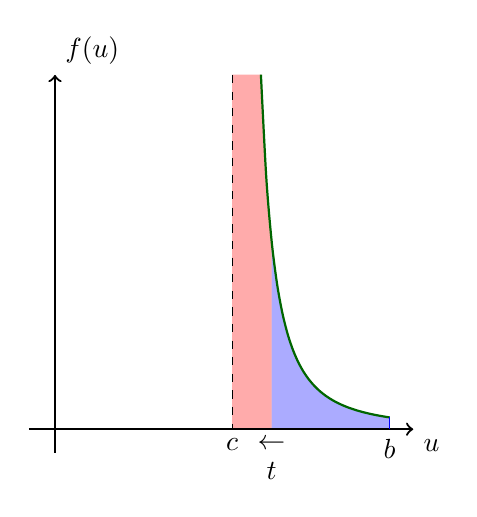
\begin{tikzpicture}[yscale=3]

	\fill[blue,opacity=0.33] plot[domain=2.75:4.25,smooth] (\x,{0.2 / ((\x - 2.25) * (\x - 2.25)}) -- (4.25,0) -- (2.75,0) -- cycle;

	\fill[red,opacity=0.33] plot[domain=2.615:2.75,smooth] (\x,{0.2 / ((\x - 2.25) * (\x - 2.25)}) -- (2.75,0) -- (2.25,0) -- (2.25,1.501) -- (2.615,1.501) -- cycle;

	% axes
	\draw[->,thick] (\xmin,0) -- (\xmax,0) node[below right] {$u$};
	\draw[->,thick] (0,\ymin) -- (0,\ymax) node[above right] {$f(u)$};

	\draw[thick, green!40!black, domain=2.615:4.25,smooth] plot (\x,{0.2 / ((\x - 2.25) * (\x - 2.25)});

	\draw[blue,thin] (4.25,0.05) -- (4.25,0) node[black,below] {$b$};
	\draw[dashed] (2.25,\ymax) -- (2.25,0) node[below] {$c$};
	\node[below] at (2.75,0) {$\leftarrow$};
	\node[below] at (2.75,-0.1) {$t$};

\end{tikzpicture}
